\documentclass[11pt]{article} % scrbook otro formato
\usepackage[utf8]{inputenc}
\usepackage[spanish,es-tabla,es-nodecimaldot]{babel}

% Paquetes

\usepackage{amsmath}
\usepackage{amsthm}
\usepackage{amsfonts}
\usepackage{amssymb}
\usepackage{makeidx}
\usepackage{graphicx}
\usepackage{lmodern}
%\usepackage{kpfonts}
\usepackage{fancyhdr}
\usepackage{geometry}
\usepackage{lastpage}
\usepackage{array} % Para fjar tamaño de columnas
\RequirePackage{siunitx}
\usepackage{extramarks} % Para poder usar firstleftmarks
\usepackage[version=4]{mhchem} % Para poder usar formulas de reacciones nucleares
\usepackage{xcolor}
%\usepackage{newtxtext, newtxmath} % Cambia la fuente (pero mola)

%##############################################################################
%######### Ponemos el decimal con . ###########################################
%##############################################################################

\sisetup{output-decimal-marker={.},
	% exponentes ------------------------
	%exponent-mode=threshold,
	%exponent-thresholds=-3:2, % non usar exponentes 10^{-2,-1, 0, 1}
	% redondear -------------------------
	% round-mode=figures, % cifras sig
	% round-mode=places, % cantos decimales
	round-mode=uncertainty, % cifras sig da incerteza (necesario usar erro)
	round-precision=2,
	uncertainty-mode = separate,
	print-unity-mantissa=false,
	% unidades --------------------------
	inter-unit-product = \ensuremath{{}\cdot{}}, % separacion entre unidades
	% per-mode=power-positive-first, % so furrula con metodo interpretado puro
	inline-per-mode=single-symbol,
	display-per-mode=fraction,
}

%##############################################################################
%######### Para codigo python #################################################
%##############################################################################

\definecolor{codegreen}{rgb}{0,0.6,0}
\definecolor{codegray}{rgb}{0.5,0.5,0.5}
\definecolor{codepurple}{rgb}{0.58,0,0.82}
\definecolor{backcolour}{rgb}{0.95,0.95,0.92}

\usepackage{listings}


%\lstdefinestyle{mystyle}{	backgroundcolor=\color{backcolour},   	commentstyle=\color{codegreen},	keywordstyle=\color{magenta},	numberstyle=\tiny\color{codegray},	stringstyle=\color{codepurple},	basicstyle=\ttfamily\footnotesize,	breakatwhitespace=false,         	breaklines=true,                 	captionpos=b,                    	keepspaces=true,                 	numbers=left,                    	numbersep=5pt,                  	showspaces=false,                	showstringspaces=false,	showtabs=false,                  	tabsize=2}

%\lstset{style=mystyle}
%\usepackage{background}     % Para manejar el fondo


%##############################################################################
%######### Tipo de fuente #################################################
%##############################################################################

%\usepackage{kpfonts}

%\usepackage{helvet} 
%\renewcommand{\familydefault}{\sfdefault}.

%\usepackage{fontspec} % Paquete necesario para seleccionar fuentes
%\setmainfont{Verdana} % Cambia la fuente principal a Verdana


%##############################################################################
%######### Geometría #################################################
%##############################################################################

\geometry{a4paper, total={152mm,237mm}, left=31mm, top=30mm}



%##############################################################################
%######### Formatos capítulo #################################################
%##############################################################################

%\usepackage[lmodern]{quotchap}
%\usepackage[Bjornstrup]{fncychap}

% Para el Bjornstrup
%\ChNumVar{\fontsize{76}{80}\usefont{OT1}{pzc}{m}{n}\selectfont}
%\ChTitleVar{\raggedright\Huge\sffamily\bfseries}


%##############################################################################
%######### Hiperreferenias #################################################
%##############################################################################


\usepackage[colorlinks=true,allcolors=blue]{hyperref} % Crea las


%##############################################################################
%######### Formato de pagina #################################################
%##############################################################################

%\renewcommand{\chaptermark}[1]{\markboth{\chaptername\ \thechapter.\ #1}{}}
\renewcommand{\sectionmark}[1]{\markright{\thesection.\ #1}}

\setlength{\headsep}{27pt} % Distancia entre la cabezera y el texto
\setlength{\footskip}{30pt} % Distancia entre el pie de pagina y el texto
\pagestyle{fancy}
\fancyhf{}
\fancyhead[LE]{\leftmark} % L,R,C-> left, right, center [LE,RO]
\fancyhead[RO]{\leftmark} % E,O -> even (par), odd (impar)
\fancyhead[LO,RE]{Daniel Vázquez Lago}
\fancyfoot[CE,CO]{\thepage}
\renewcommand{\headrulewidth}{1pt} % Cambiamos el grosor de la linea de arriba
\renewcommand{\footrulewidth}{0pt}



%##############################################################################
%#########  Modificar caption #################################################
%##############################################################################

\usepackage[font=small, justification=centering]{caption}  % Configura las captions



%##############################################################################
%######### Comandos propios #################################################
%##############################################################################

\newcommand{\parentesis}[1]{\left( #1  \right)} 
\newcommand{\parciales}[2]{\frac{\partial #1}{\partial #2}}
\newcommand{\pparciales}[2]{\parentesis{\parciales{#1}{#2}}}
\newcommand{\ccorchetes}[1]{\left[ #1  \right]}
\newcommand{\D}{\mathrm{d}}
\newcommand{\derivadas}[2]{\frac{\D #1}{\D #2}}

\newcommand{\tquad}{\quad \quad \quad}
\newcommand{\vnabla}{\vec{\nabla}}

\newcommand{\Ocal}{\mathcal{O}}
\newcommand{\Ncal}{\mathcal{N}}
\newcommand{\Hcal}{\mathcal{H}}

\newcommand{\logd}{\log_{10}}

\newcommand{\eV}{\text{eV}}
\newcommand{\cm}{\text{cm}}
\newcommand{\cmm}{\text{cm}^{-1}}
\newcommand{\fm}{\text{fm}}
\newcommand{\He}{\text{He}}
\newcommand{\p}{\text{p}}
\newcommand{\e}{\text{e}}
\newcommand{\cte}{\text{cte}}


% Comandos vectoriales

\newcommand{\an}{\mathbf{a}}
\newcommand{\bn}{\mathbf{b}}
\newcommand{\dn}{\mathbf{d}}
\newcommand{\jn}{\mathbf{j}}
\newcommand{\lnn}{\boldsymbol{\ell}}
\newcommand{\lnnn}{\boldsymbol{l}}
\newcommand{\kn}{\mathbf{k}}
\newcommand{\pn}{\mathbf{p}}
\newcommand{\qn}{\mathbf{q}}
\newcommand{\rn}{\mathbf{r}}
\newcommand{\sn}{\mathbf{s}}
\newcommand{\un}{\mathbf{u}}
\newcommand{\vn}{\mathbf{v}}
\newcommand{\xn}{\mathbf{x}}
\newcommand{\yn}{\mathbf{y}}
\newcommand{\qndot}{\dot{\qn}}

\newcommand{\unovec}{\vec{\mathbf{1}}}

\newcommand{\alphan}{\boldsymbol{\alpha}}
\newcommand{\sigman}{\boldsymbol{\sigma}}
\newcommand{\pin}{\boldsymbol{\pi}}


\newcommand{\An}{\mathbf{A}}
\newcommand{\Bn}{\mathbf{B}}
\newcommand{\En}{\mathbf{E}}
\newcommand{\Gn}{\mathbf{G}}
\newcommand{\Jn}{\mathbf{J}}
\newcommand{\Kn}{\mathbf{K}}
\newcommand{\Ln}{\mathbf{L}}
\newcommand{\Rn}{\mathbf{R}}
\newcommand{\Sn}{\mathbf{S}}
\newcommand{\Tn}{\mathbf{T}}
\newcommand{\In}{\mathbf{I}}

\newcommand{\hnn}{\hat{\mathbf{n}}}
\newcommand{\hnr}{\hat{\mathbf{r}}}
\newcommand{\hnz}{\hat{\mathbf{z}}}
\newcommand{\hnx}{\hat{\mathbf{x}}}
\newcommand{\hny}{\hat{\mathbf{y}}}
\newcommand{\hnu}{\hat{\mathbf{u}}}
\newcommand{\hnR}{\hat{\mathbf{R}}}
\newcommand{\hnv}{\hat{\mathbf{v}}}
\newcommand{\hnk}{\hat{\mathbf{k}}}
\newcommand{\hni}{\hat{\mathbf{i}}}
\newcommand{\hnj}{\hat{\mathbf{j}}}
\renewcommand{\hnk}{\hat{\mathbf{k}}}





%##############################################################################
%######### Teoremas/definiciones #################################################
%##############################################################################

%\theoremstyle{definition}
%\newtheorem{definition}{Definición}[chapter]
%\theoremstyle{theorem}
%\newtheorem{theorem}{Teorema}[chapter]




%##############################################################################
%######### Referncia para euccaiones y figuras ################################
%##############################################################################

%\numberwithin{equation}{section}
%\numberwithin{figure}{section}




%##############################################################################
%######### Documento #################################################
%##############################################################################


\author{Daniel Vazquez Lago}
\title{Simulación en física de materiales}


\begin{document}	
	
\maketitle
\newpage
\tableofcontents
\section{Objetivos}

El objetivo de esta segunda entrega de la asignatura es llegar a la posición de equilibrio de un sistema de 500 partículas, con una densidad $\rho=0.5$ y una energía $E=575$ (variables reducidas) a partir de una posición inicial fcc. Para saber si hemos alcanzado una configuración de equilibrio usaremos dos métodos, que de manera muy escueta son: 

\begin{itemize}
	\item La energía total se conserva con el tiempo, con un promedio estable (aunque haya oscilaciones estas deben ser muy pequeñas).
	\item La distribución de las velocidades deben verificar distribuciones de Maxwell, así como un valor medio nulo $\langle v_i \rangle = 0$. 
\end{itemize}
Sin embargo para llegar al equilibrio primero debemos avanzar en el tiempo, es decir, hacer una simulación. Consecuentemente la primera parte de este proyecto será ver como se hace la evolución temporal, por qué de esa forma y no de otra; para luego ver como la implementamos, ver los primeros resultados y posteriormente analizar de los resultados con los dos métodos y ver si se verifica o no la condición de equilibrio. 


\section{Simulación}

En esta sección vamos a ver como se hace la simulación, esto es, como calculamos la posición, velocidad... en la configuración $t+\Delta t$ a partir de los datos en $t$ (o anteriores, esto es, $t  - \Delta t, \ t - 2 \Delta t$). Primero haremos la introducción teórica, para luego ver la implementación práctica.

\subsection{Introducción teórica}

Para conocer la posición de las partículas en el instante de $t + \Delta t$, si $\Delta t$ es suficientemente pequeña, podemos desarrollar la serie de Taylor de $\rn(t+\Delta t)$

\begin{eqnarray}
	\rn(t+\Delta) = \rn (t) + \dot{\rn} (t) \Delta t + \frac{1}{2} \ddot{\rn} (t) (\Delta T)^2 + \frac{1}{6} \dddot{\rn} (t) (\Delta T)^3 + \ldots
\end{eqnarray}
Conocidos los valores de $\rn,\dot{\rn}$, $\ddot{\rn}...$ podremos calcular la nueva posición. Sin embargo esto nos lleva a dos preguntas ¿A qué nos referimos con $\Delta t$ suficientemente pequeña?¿Qué valor le asignamos a las variables $\dot{\rn}...$? 


La segunda tiene una respuesta bien sencilla: para conocer los valores de  supongamos que tenemos un sistema completamente aislado, del que solo conocemos el hamiltoniano $\Hcal$, dado por la energía cinética y un potencial que solo depende de la posición:

\begin{eqnarray}
	\Hcal = \sum_{i=1} \frac{\pn_i^2}{2m} + \varphi (\rn_i)
\end{eqnarray}
Si definimos la velocidad como $\pn=m\vn$ y la aceleración como $\ddot{\rn}_i = \an_i$, tenemos que:

\begin{eqnarray}
	\dot{\rn}_i = \parciales{\Hcal}{\pn_i} = \frac{\pn_i}{m} = \vn_i
\end{eqnarray}

\begin{eqnarray}
	\dot{\pn}_i = - \parciales{\Hcal}{\rn_i} \Rightarrow  m \ddot{\rn}_i = - \parciales{\varphi(\rn_i)}{\rn_i} \Rightarrow \an_i =  - \frac{1}{m} \parciales{\varphi(\rn_i)}{\rn_i}
\end{eqnarray}
De esto es trivial deducir que si conocemos la posición de $t+\Delta t$, conocemos las aceleraciones $\an_i$, ya que el potencial $\varphi(\rn_i)$ solo depende la posición. Recordemos que usamos variables reducidas, esto es $m=1$.

Aunque parezca que lo que acabamos de hacer es trivial, en realidad no lo es, ya que de tener otro tipo de hamiltoniano (por ejemplo el de una configuración PVT) estas ecuaciones no tendrían que ser así (apareciendo factores). Es importante ver que efectivamente, se verifica que 

\begin{eqnarray}
	\dot{\rn}_i = \vn_i \tquad \an_i = - \parciales{\varphi(\rn_i)}{\rn_i}
\end{eqnarray}
Ahora la pregunta que nos hacemos es que 


\subsection{Implementación en Fortran}

\subsection{Resultados}

Una vez corremos la simulación, obtenemos los resultados de la energía que vemos en la figura \ref{Fig:01}. 


\begin{figure}[h!] \centering
	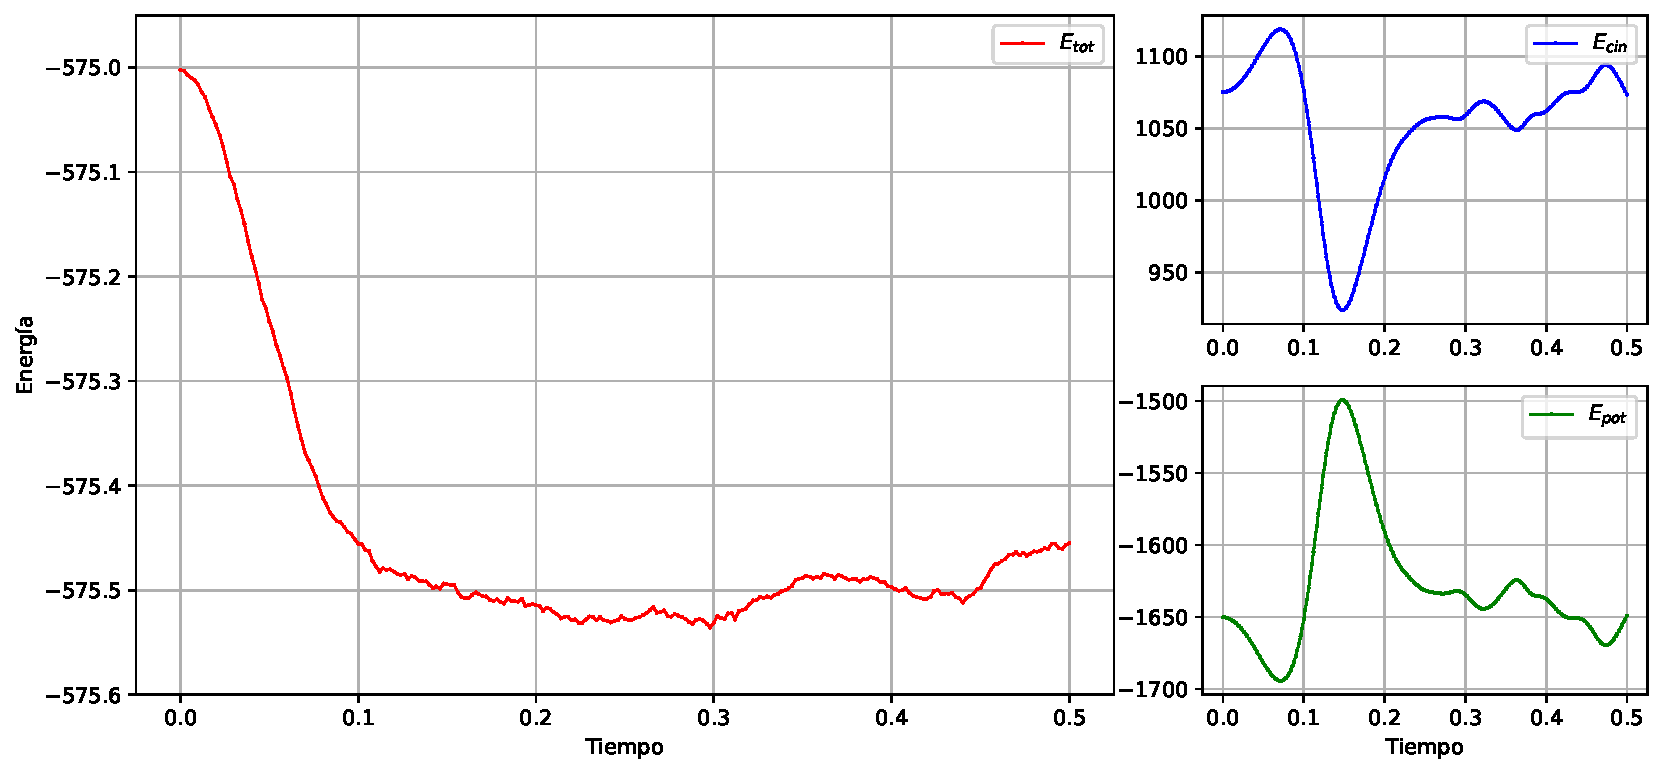
\includegraphics[width=0.9\textwidth]{../../Graficas/Et-equilibra.pdf}
	\caption{evolución de la energía total desde la configuración fcc y 5000 pasos.}
	\label{Fig:01}
\end{figure}	

Tras subir la energía a 575 mediante el mismo algoritmo usado para en la colocación inicial para reescalar las velocidades (adecuándose a la energía cinética que necesitamos para que $E=575$) y asegurándonos que el momento total se mantenga cero, volvemos a hacer la simulación. A diferencia de la anterior inicialización, en esta no habrá un salto de energía tan llamativo, ya que al haber dejado que ocurrieran 5000 pasos, la colocación de las partículas ya no es simétrica, estando mucho más cerca del equilibrio, por lo que haremos $\num{5e5}$. Una vez con la simulación hecha, podremos ver si de verdad hemos llegado al equilibrio, con los métodos propuestos en el siguiente apartado. 



\begin{figure}[h!] \centering
	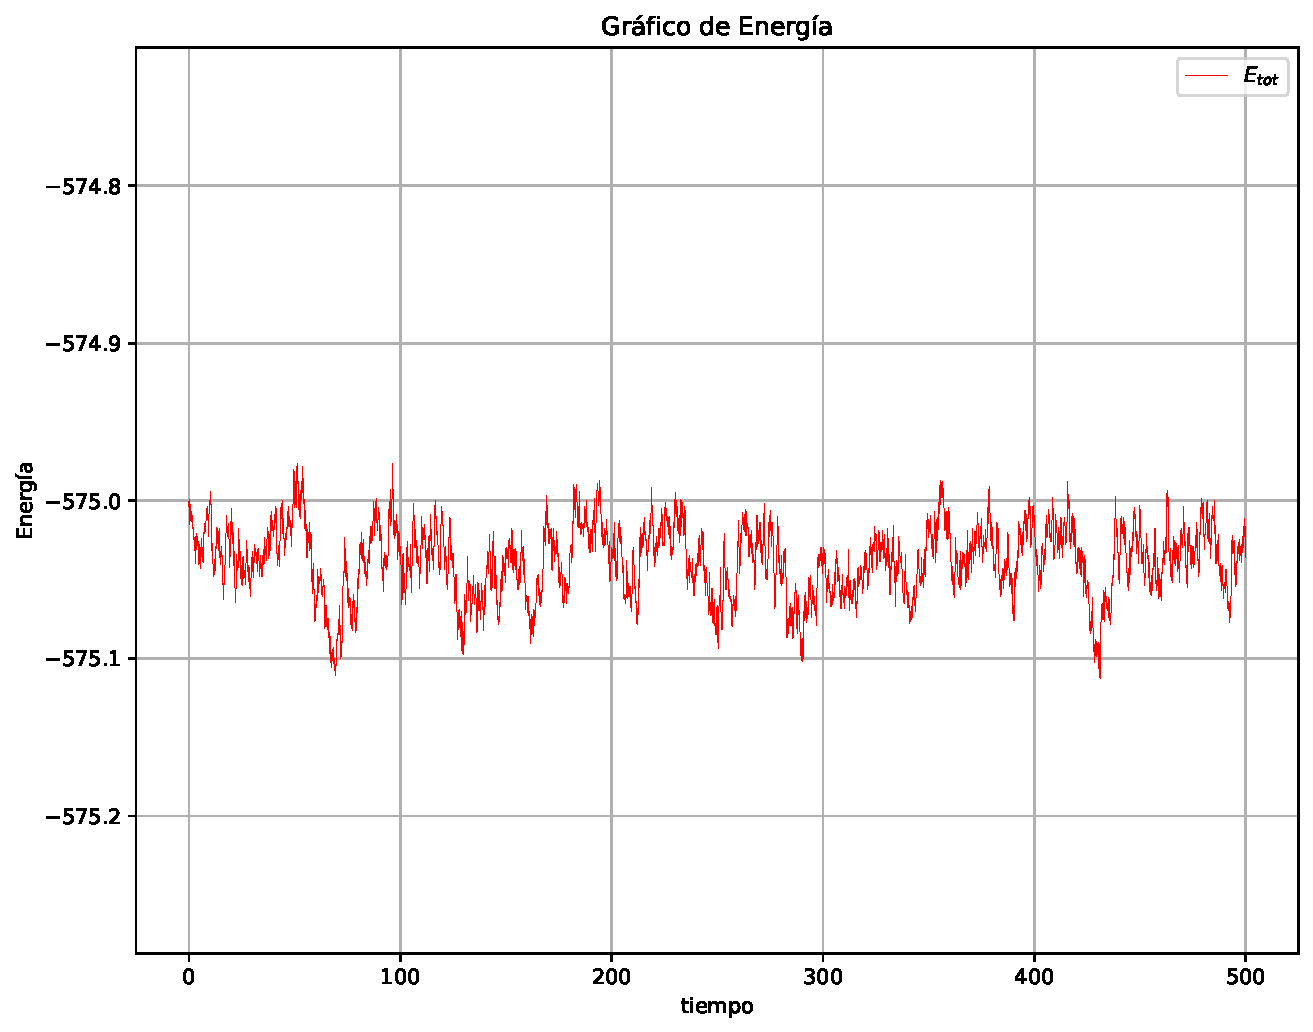
\includegraphics[width=0.9\textwidth]{../../Graficas/Et-equilibra-500K.pdf}
	\caption{evolución de la energía total 500000 pasos.}
	\label{Fig:04}
\end{figure}	


\section{Equlibración}

En este apartado discutiremos cuales son los métodos para ver si la configuración ha llegado al equilibrio desde una perspectiva teórica inicialmente (viendo por qué estos métodos son válidos) para luego ver como los implementamos, para en el apartado de resultados ver si realmente hemos llegado al equilibrio. 

\subsection{Teoría}

\cite{Haile}

\subsubsection{Verificación con la energía}

La verificación con la energía es la única 


\subsubsection{Verificación con la velocidad}

\subsubsection{Verificación con la H de Boltzmann}

\subsection{Implementación en Fortran}

\subsection{Resultados}

Veamos cada uno de los resultados. 


\begin{figure}[h!] \centering
	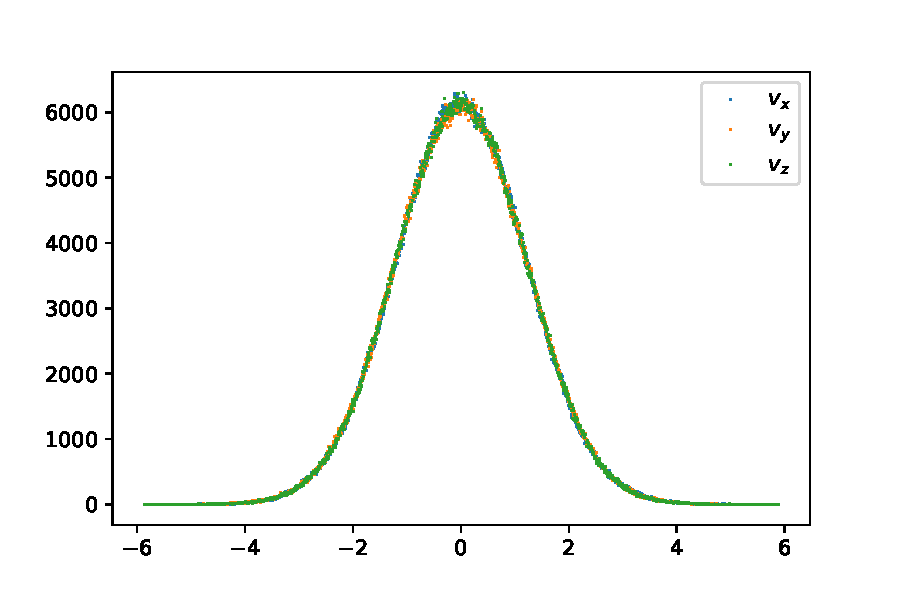
\includegraphics[width=0.8\textwidth]{../../Graficas/Velocidades_histo.pdf}
	\caption{distribución de la velocidad tras los 500000 pasos.}
	\label{Fig:07}
\end{figure}	


\section{Conclusiones}

\section{Organización}

En este proyecto hemos usado los siguientes archivos, en los que podremos encontrar:


\section{Gráficas}


\begin{figure}[h!] \centering
	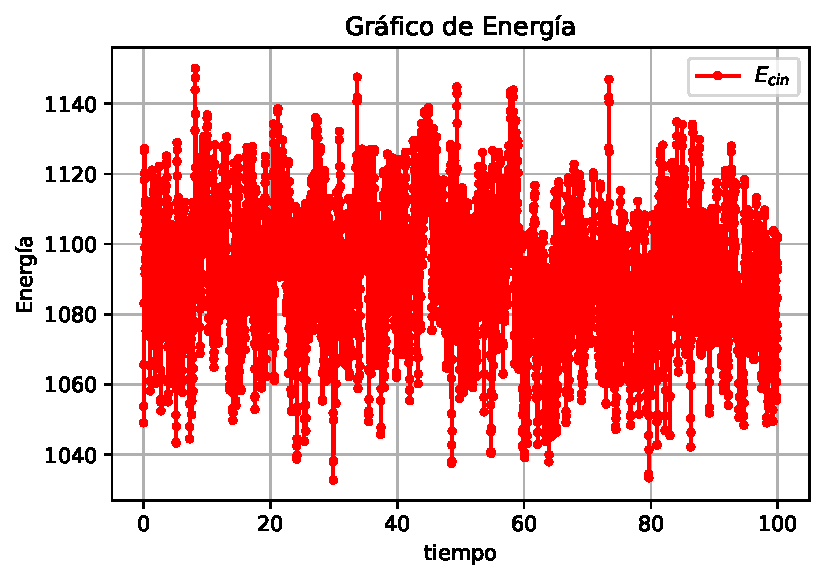
\includegraphics[width=0.9\textwidth]{../../Graficas/Ecin-equilibra.pdf}
	\caption{evolución de la energía cinética desde la configuración fcc y 5000 pasos.}
	\label{Fig:02}
\end{figure}	

\begin{figure}[h!] \centering
	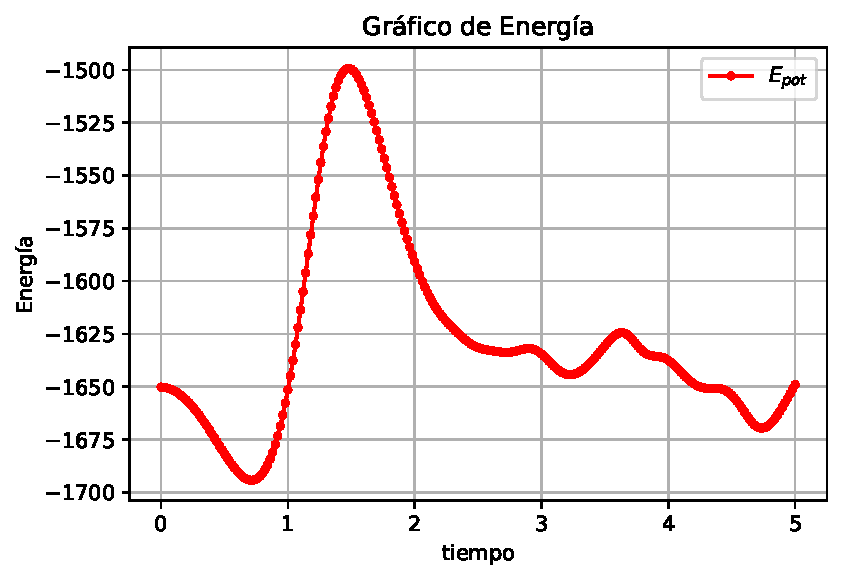
\includegraphics[width=0.9\textwidth]{../../Graficas/Epot-equilibra.pdf}
	\caption{evolución de la energía potencial desde la configuración fcc y 5000 pasos.}
	\label{Fig:03}
\end{figure}	

\begin{figure}[h!] \centering
	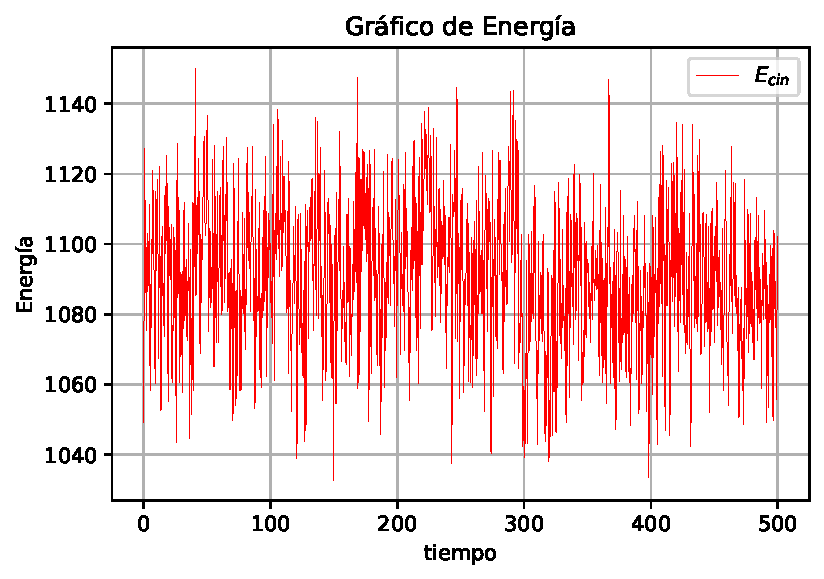
\includegraphics[width=0.9\textwidth]{../../Graficas/Ecin-equilibra-500K.pdf}
	\caption{evolución de la energía cinética 500000 pasos.}
	\label{Fig:05}
\end{figure}	

\begin{figure}[h!] \centering
	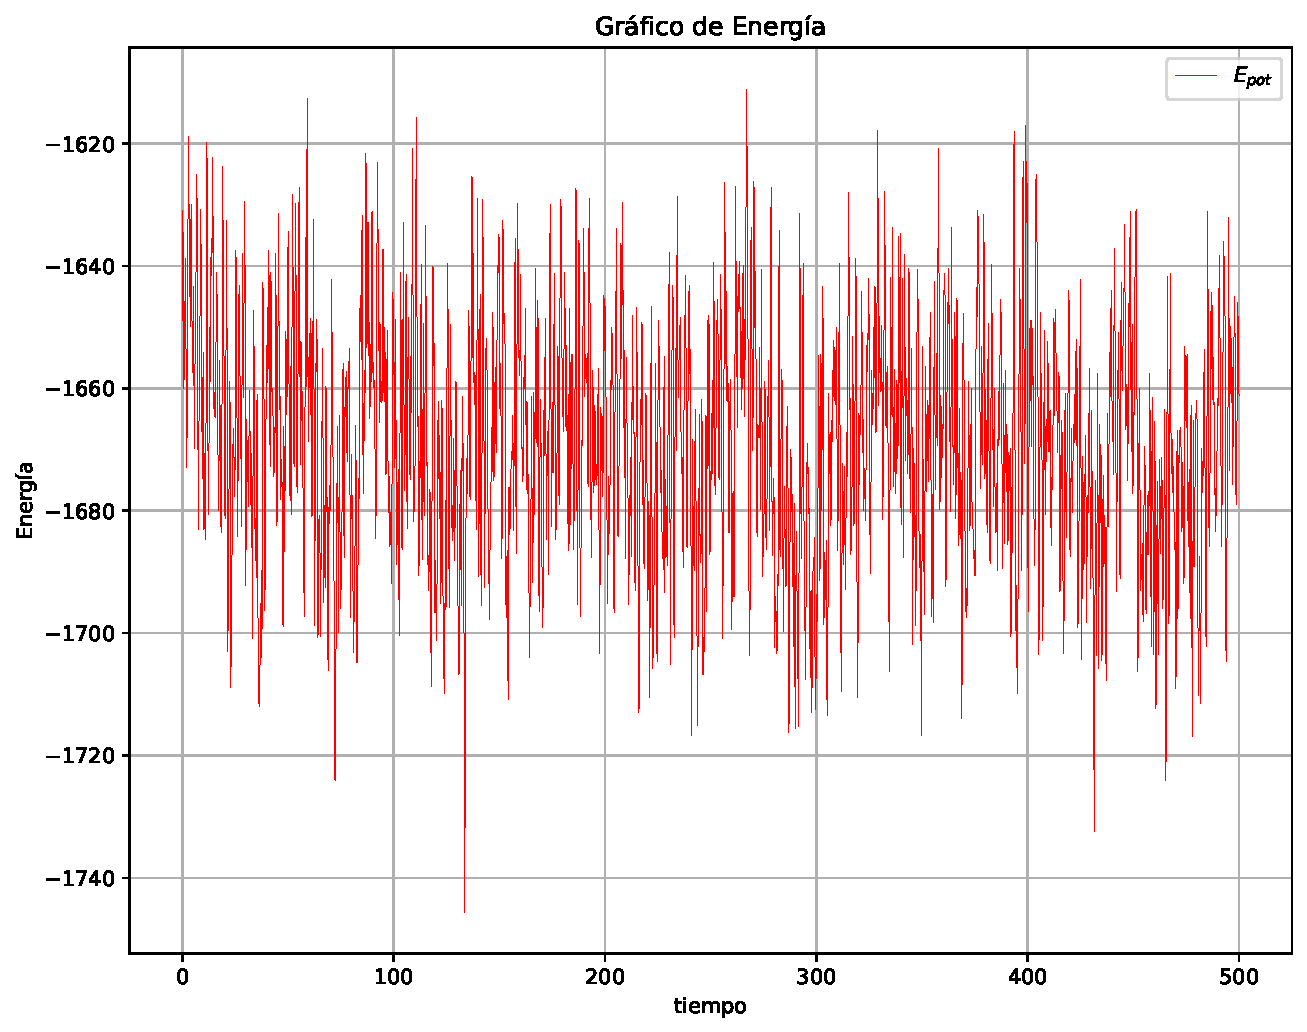
\includegraphics[width=0.9\textwidth]{../../Graficas/Epot-equilibra-500K.pdf}
	\caption{evolución de la energía potencial 500000 pasos.}
	\label{Fig:06}
\end{figure}	
\bibliography{Bibliografia.bib}
\bibliographystyle{unsrt}
	
\end{document}	
